%!TEX root = master.tex

\section{Umsetzung}

\subsection{Theorie}
\subsection{Implementierung}

\begin{frame}
  \frametitle{Theorie}

  \setbeamertemplate{itemize items}[circle]
  \begin{itemize}  
    \item Die Daten werden vor dem Transfer in kleine Teile (Chunks) geteilt. Es muss mindestens so viele Chunks geben, wie es Peers im Netzwerk gibt.

    \item Der Super-Peer verschickt disjunkte Chunks parallel an alle übrigen Peers.

    \item Jeder Peer verschickt seinen Chunk an alle anderen Peers.

    \item Es wird vereinfacht angenommen, dass jeder Peer die gleiche Uploadbandbreite hat.
  \end{itemize}	

\end{frame}




\begin{frame}
  \frametitle{Theorie}
  Wenn es genauso viele Chunks wie Peers gibt, kann man den Transfer in zwei Stufen betrachten. Peer 1 ist in diesem Fall der Super-Peer.
  \begin{itemize}
    \item Links: Alle Peers bekommen einen disjunkten Chunk vom Super-Peer. 
    \item Rechts: Die Peers schicken sich ihren eigenen Chunk gegenseitig zu. 
  \end{itemize}

  \begin{center}
    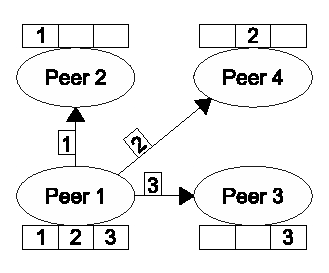
\includegraphics[width=0.4\textwidth]{fig/chunkedswarmmodel1.eps}
    \hspace{0.15\textwidth}
    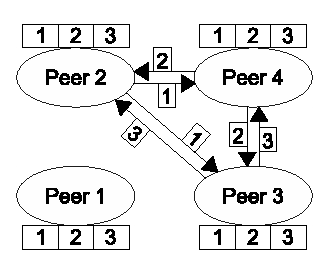
\includegraphics[width=0.4\textwidth]{fig/chunkedswarmmodel2.eps}
  \end{center}
\end{frame}


\begin{frame}
  \frametitle{Theorie}
  Das folgende Bild zeigt den zeitlichen Ablauf:
  \begin{itemize}
    \item In den ersten $T_0$ Sekunden, schickt der Super-Peer einen disjunkten Chunk an jeden Peer. Jeder Chunk ist daher $\frac{Datengr"o"se}{Anzahl}$ groß.
    \item Anschließend schickt jeder Peer seinen Chunk an die anderen beiden Peers, was $\frac{2}{3} * T_0$ Sekunden dauert.
    \item Nach $T_0 + \frac{2}{3} * T_0$ Sekunden besitzt also jeder Peer die Daten.
  \end{itemize}

  \begin{center}
    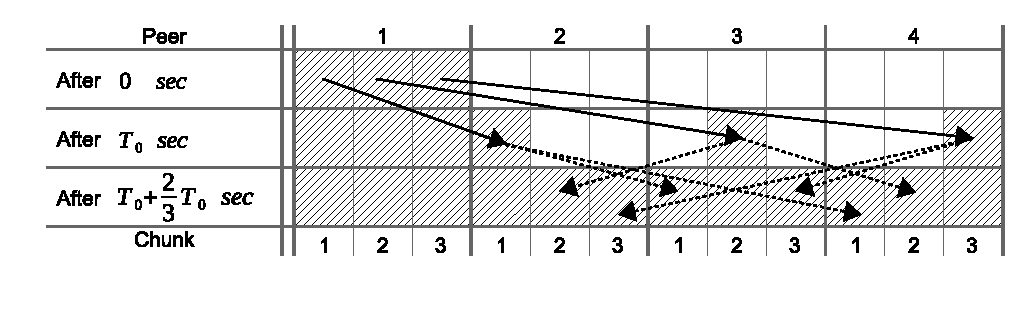
\includegraphics[width=1\textwidth]{fig/chunkedswarmformula1.eps}
  \end{center}
\end{frame}



\begin{frame}
  \frametitle{Theorie}

  \setbeamertemplate{itemize items}[circle]
  \begin{itemize}  
    \item Verdoppelt man die Anzahl der Chunks, halbiert man die Zeit zwischen $T_0$ Sekunden und dem Ende.
    \item Die allgemeine Gesamtdauer lässt sich daher mit $T(n, c) = T_0\:+\:\frac{n}{c}\:*\:\frac{n-1}{n}\:*\:T_0 = (1\:+\:\frac{n-1}{c})\:*\:T_0$ berechnen, wobei $n$ die Anzahl der Peers, jedoch ohne den Super-Peer, und $c = n\:*\:2^i, i \in \mathbb{N}_0$ die Anzahl der Chunks ist.

    \item Mit dieser Methode kann man immer unter $2 * T_0$ Sekunden kommen. Verdoppelt man die Anzahl der Chunks beliebig oft, so kann man sogar beliebig nah an $T_0$ Sekunden herankommen.
  \end{itemize} 

\end{frame}





\begin{frame}
  \frametitle{Implementierung}

  \setbeamertemplate{itemize items}[circle]
  \begin{itemize}  
    \item Mesh Topologie: Jeder Peer ist mit jedem Peer verbunden.
    \item Pull-Based: Chunks werden nur auf Wunsch übertragen.
    \item Announcements: Jeder Peer kündigt an, welche Chunks vorliegen.
    \item Automatic (Re-)Connect: Peers finden andere Peers durch Super-Peer.
  \end{itemize} 

\end{frame}

\begin{frame}
  \frametitle{Implementierung}

  \setbeamertemplate{itemize items}[circle]
  \begin{itemize}  
    \item Peer-Loss Detection: Super-Peer verschickt Chunks von Peers, die das Netzwerk verlassen haben, erneut.
    \item Jeder Peer versucht von möglichst vielen Peers gleichzeitig Chunks zu beziehen. Dies ist wichtig, da ein Pull-Based Ansatz verwendet wird.
    \item Implementiert in Java mit Netty5.
  \end{itemize} 

\end{frame}

